%% CELERIS -- Computer Physics Communications (CPiP) submission.
%% Document class: Elsevier elsarticle. Bibliography: elsarticle-num (paper.bib).
%% Build:  pdflatex paper  ->  bibtex paper  ->  pdflatex paper  ->  pdflatex paper
\documentclass[preprint,12pt]{elsarticle}

\usepackage[T1]{fontenc}
\usepackage{amsmath}
\usepackage{amssymb}
\usepackage{graphicx}
\usepackage{booktabs}
\usepackage{pifont}
\usepackage{url}

% Feature-table glyphs.
\newcommand{\yes}{\ding{51}}          % provided
\newcommand{\no}{\ding{55}}           % not provided
\newcommand{\pt}{$\sim$}              % partial / possible with user code
\newcommand{\na}{---}                 % not applicable

\journal{Computer Physics Communications}

\begin{document}

\begin{frontmatter}

\title{CELERIS: an integrated, validated RCWA pipeline for metalens
design, analysis, and fabrication layout}

\author[ucf]{Amarnath Patel\corref{cor1}}
\ead{am397421@ucf.edu}
\cortext[cor1]{Corresponding author.}
\affiliation[ucf]{organization={University of Central Florida},
                  city={Orlando}, state={FL}, country={USA}}

\begin{abstract}
Metasurfaces and metalenses --- flat optical elements built from subwavelength
scatterers (``meta-atoms'') --- are designed by (i) solving Maxwell's equations
for a periodic unit cell to build a library of meta-atom responses, (ii) mapping
a target optical phase profile onto that library, (iii) analyzing the resulting
device's optical performance, and (iv) exporting a mask layout for fabrication.
The standard rigorous electromagnetic method for step (i) is rigorous coupled-wave
analysis (RCWA), also known as the Fourier modal method (FMM). \textbf{CELERIS} is
a from-scratch, validated implementation of this \emph{entire} workflow in a single
native package. It couples a C++23 RCWA engine (1D and 2D-vectorial, with Li/Liu--Fan
Fourier factorization and a Redheffer S-matrix stack) to a meta-atom library builder,
a phase-mapping and inverse-design layer (including achromatic and Pancharatnam--Berry
designs), a full optical analysis battery (Strehl ratio, PSF, MTF, wavefront/Zernike,
through-focus, chromatic, field-resolved, and tolerance analyses), GPU-accelerated
far-field propagation, and fabrication-ready GDSII export. It is scriptable from C++,
a command-line interface, and Python (via pybind11), and ships with a desktop GUI.
Correctness is enforced by a locked self-test suite (20+ cases) cross-checked against
closed-form physics (Fresnel/TMM, effective-medium theory), energy conservation, and
independent RCWA solvers (\texttt{grcwa} and Stanford~S$^4$), and the full pipeline is
demonstrated by reproducing two canonical published TiO$_2$ metalenses end to end.
\end{abstract}

\begin{keyword}
metasurface \sep metalens \sep rigorous coupled-wave analysis \sep
Fourier modal method \sep inverse design \sep GDSII
\end{keyword}

\end{frontmatter}

%% ---------------------------------------------------------------------------
\section*{Program summary}
\noindent\emph{(CPC-mandatory block; exact fields are entered on the submission form.)}
\begin{description}
\item[Program title:] CELERIS
\item[Licensing provisions:] Apache License 2.0
\item[Permanent archive:] Zenodo (v1.0.0): \url{https://doi.org/10.5281/zenodo.21891346};
      concept DOI (always latest version): \url{https://doi.org/10.5281/zenodo.21891345}
\item[Programming languages:] C++23 (engine), CUDA (optional GPU far-field kernel),
      Python (pybind11 bindings)
\item[Nature of problem:] Designing a metalens/metasurface requires solving Maxwell's
      equations for periodic subwavelength unit cells, assembling a meta-atom library,
      mapping a target optical phase profile onto it, analyzing the resulting device's
      optical performance, and exporting a fabrication mask --- a multi-stage workflow
      that existing RCWA solvers do not provide end to end.
\item[Solution method:] Rigorous coupled-wave analysis / Fourier modal method (1D and
      2D-vectorial) with Li/Liu--Fan Fourier factorization and a Redheffer S-matrix
      layer recursion, wrapped in a library builder, a phase-mapping / inverse-design
      layer (including achromatic and Pancharatnam--Berry recipes), an optical analysis
      battery, GPU-accelerated far-field propagation, and GDSII layout export.
\item[Dependencies:] Eigen (header-only, fetched at configure time); optional Intel MKL
      and CUDA for acceleration; pybind11 for the Python module. Validated against
      \texttt{grcwa} and Stanford~S$^4$.
\item[Restrictions:] Scope is metalenses/metasurfaces via RCWA (not FDTD or ray
      tracing). The modal eigensolve runs on the CPU; the GPU accelerates far-field
      propagation only.
\item[Operating systems:] Linux and Windows (CPU build has no external runtime
      dependencies).
\end{description}

%% ---------------------------------------------------------------------------
\section{Statement of need}
Existing open-source RCWA codes --- S$^4$~\cite{liu2012s4}, RETICOLO~\cite{reticolo},
\texttt{grcwa}~\cite{grcwa}, TORCWA~\cite{torcwa}, \texttt{fmmax}~\cite{fmmax},
\texttt{meent}~\cite{meent} --- are \emph{solver kernels}: they compute the
electromagnetic response of a given periodic structure. Turning a solver into a
\emph{fabricated, analyzed metalens} still requires the user to hand-assemble the
surrounding workflow: sweeping a meta-atom library, mapping a phase profile onto it,
propagating to a focal plane, computing imaging metrics, running fabrication-tolerance
studies, and emitting a GDSII layout. Each researcher re-implements this scaffolding,
and the glue code is rarely validated or shared.

CELERIS provides that pipeline as a single validated tool. The target audience is
metasurface and metalens researchers who need to go from an optical specification
(focal length, aperture, wavelength, material) to a fabrication-ready, performance-
characterized design without stitching together a solver, a plotting stack, and a
layout tool. The contribution is not a new solver kernel but the \textbf{integration}
--- solver $\to$ library $\to$ design $\to$ analysis $\to$ layout --- validated
end to end against published devices.

%% ---------------------------------------------------------------------------
\section{State of the field}
Table~\ref{tab:compare} positions CELERIS against widely used RCWA/FMM codes. CELERIS
deliberately \emph{does not} compete on automatic differentiation (see Limitations);
it competes on the integrated design--analysis--fabrication workflow, which the solver
kernels do not provide.

\begin{table*}[t]
\centering
\caption{Feature comparison (\yes~= provided, \pt~= partial/possible with user code,
\no~= not provided). Verified against each tool's documentation/publication; released
versions evolve, so cells should be re-checked at submission.}
\label{tab:compare}
\footnotesize
\setlength{\tabcolsep}{4pt}
\resizebox{\textwidth}{!}{%
\begin{tabular}{lccccccc}
\toprule
Feature & S$^4$ & RETICOLO & grcwa & TORCWA & fmmax & meent & \textbf{CELERIS} \\
\midrule
Language                        & C++/Lua/Py & MATLAB & Python & PyTorch & JAX & np/JAX/torch & \textbf{C++/Py} \\
License                         & GPL & (MATLAB) & GPL & \na & MIT & MIT & \textbf{Apache-2.0} \\
1D + 2D-vectorial RCWA          & \yes & \yes & \yes & \yes & \yes & \yes & \textbf{\yes} \\
Native GPU (full solve)         & \no & \no & \no & \yes & \yes & \yes & \textbf{\no~(far-field only)} \\
Automatic differentiation       & \no & \no & \yes & \yes & \yes & \yes & \textbf{\no~(FD; adjoint planned)} \\
Arbitrary meta-atom shapes      & \yes & \yes & \yes & \yes & \yes & \yes & \textbf{\yes} \\
Integrated metalens \emph{design} & \no & \no & \pt & \pt & \pt & \pt & \textbf{\yes} \\
Optical \emph{analysis battery} & \no & \pt & \no & \no & \no & \no & \textbf{\yes} \\
Achromatic + PB design          & \no & \no & \no & \no & \no & \no & \textbf{\yes} \\
Fabrication-ready GDSII export  & \no & \no & \no & \no & \no & \no & \textbf{\yes} \\
Published-device reproductions  & \na & \na & \na & \na & \na & \na & \textbf{\yes} \\
Desktop GUI                     & \no & \no & \no & \no & \no & \no & \textbf{\yes} \\
\bottomrule
\end{tabular}%
}
\end{table*}

We state the trade-off plainly: the GPU/autodiff-native solvers (TORCWA, fmmax, meent)
are \emph{stronger solver kernels} --- they run the full modal solve on the GPU with
automatic differentiation, whereas CELERIS GPU-accelerates only far-field propagation
and optimizes by finite differences (an analytic adjoint is planned). CELERIS's
contribution is orthogonal: it is the only tool that wraps the solver in a complete,
validated \textbf{design $\to$ analysis $\to$ fabrication} workflow --- integrated
design, the optical analysis battery, achromatic/Pancharatnam--Berry recipes, GDSII
export, published-device reproductions, and a GUI --- none of which the solver kernels
provide.

%% ---------------------------------------------------------------------------
\section{Software design}
\begin{itemize}
\item \textbf{Engine (\texttt{celeris\_core}, C++23).} 1D RCWA (TE/TM, multilayer,
      S-matrix) and 2D-vectorial RCWA. The 2D solver uses the Li/Liu--Fan inverse-rule
      Fourier factorization~\cite{li1996} for axis-aligned rectangles (correct
      convergence, energy conserved to machine precision) and a stable Laurent
      factorization for arbitrary sampled shapes. Layer coupling uses a Redheffer
      S-matrix recursion~\cite{redheffer1962,rumpf2011}. The dense complex linear
      algebra runs on Eigen (header-only), optionally routed through Intel MKL.
\item \textbf{Design.} A library builder sweeps meta-atom geometry; phase profiles
      (focusing, vortex/OAM, deflector, axicon, quadratic wide-FOV, freeform) drive both
      a propagation-phase path and an exact geometric (Pancharatnam--Berry) path.
      Achromatic design engineers group delay across a band via dispersive libraries
      (fill$\times$height, single-etch shape variety, and a PB variant).
\item \textbf{Analysis.} Strehl/FWHM/encircled energy, PSF, wavefront
      (OPD/Zernike/Mar\'echal), MTF, through-focus/caustic, chromatic, spot-vs-field,
      full-field grid, tolerance, birefringence, and per-order efficiency/absorption
      budgets.
\item \textbf{Acceleration.} The far-field Rayleigh--Sommerfeld propagation --- a dense
      (pixels $\times$ pillars) reduction --- runs as a CUDA kernel (static runtime;
      CPU auto-fallback when no device is present). The RCWA eigensolve itself remains
      on the CPU (see Limitations). The CUDA build is cross-platform (Linux and Windows).
\item \textbf{Interfaces.} A CLI (\texttt{design}, \texttt{pbdesign},
      \texttt{achromatic}, \texttt{reproduce}, \texttt{selftest}, \ldots), Python
      bindings (pybind11; \texttt{pip install .}), and a Dear ImGui desktop GUI.
\end{itemize}

%% ---------------------------------------------------------------------------
\section{Validation}
Correctness is locked by a self-test suite of 20+ cases, cross-checked against:
closed-form Fresnel/TMM and Bragg-mirror results; effective-medium theory in the
deep-subwavelength limit; strict energy conservation ($R+T+A = 1$ to $10^{-6}$); and
two independent RCWA solvers, \texttt{grcwa}~\cite{grcwa} and Stanford~S$^4$
\cite{liu2012s4} (the field-standard FMM reference). The suite runs green on Linux
(GCC) and is enforced by continuous integration.

Running CELERIS and S$^4$ on an \emph{identical} freestanding $n=1.5$ binary grating
($\Lambda = 0.3~\mu$m, fill 0.5, thickness $0.5~\mu$m, $\lambda = 0.5~\mu$m, normal
incidence), the zeroth-order transmittance agrees to $7\times10^{-8}$ (TE) at $M=40$
(converging $10^{-5}\!\to\!10^{-7}$ with Fourier order), and to $3\times10^{-4}$ (TM),
the latter limited by the well-known slower TM Fourier convergence exhibited by
\emph{both} solvers. This case also equals \texttt{grcwa}'s $0.93333$ to $\sim10^{-6}$
--- a three-way agreement. The comparison is reproducible via
\texttt{paper/validation/s4\_crosscheck.py} and shown in Fig.~\ref{fig:validation}.

\begin{figure}[t]
\centering
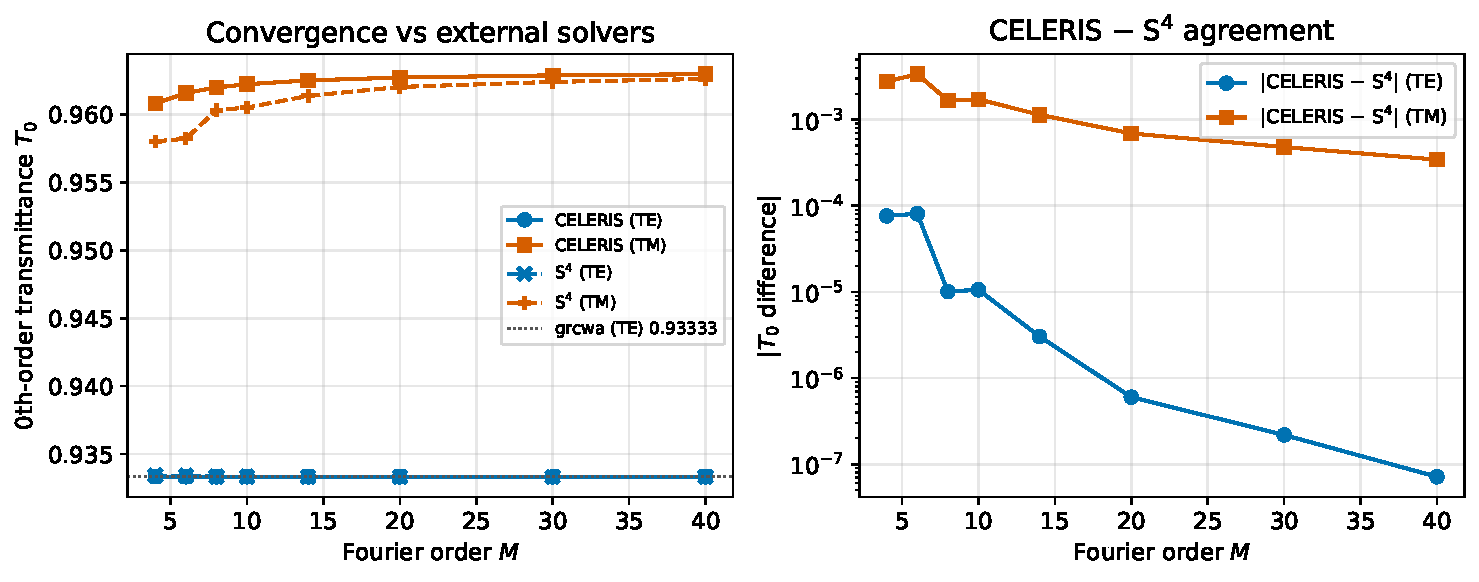
\includegraphics[width=\textwidth]{figures/fig_validation.pdf}
\caption{CELERIS vs Stanford~S$^4$ on an identical freestanding grating. Left:
0th-order transmittance vs Fourier order $M$ --- CELERIS (TE) and S$^4$ (TE) sit on
\texttt{grcwa}'s $0.93333$. Right: the CELERIS$-$S$^4$ difference falls to
$7\times10^{-8}$ (TE); TM converges more slowly for both, as expected.}
\label{fig:validation}
\end{figure}

The end-to-end pipeline is exercised in Figs.~\ref{fig:library}--\ref{fig:psf}: sweeping
a TiO$_2$ square-pillar's fill builds the phase library (Fig.~\ref{fig:library}), and
designing an NA${\approx}0.2$ focusing lens from it yields a diffraction-limited focal
spot --- FWHM equal to $\lambda f/D$ to three figures (Fig.~\ref{fig:psf}).

\begin{figure}[t]
\centering
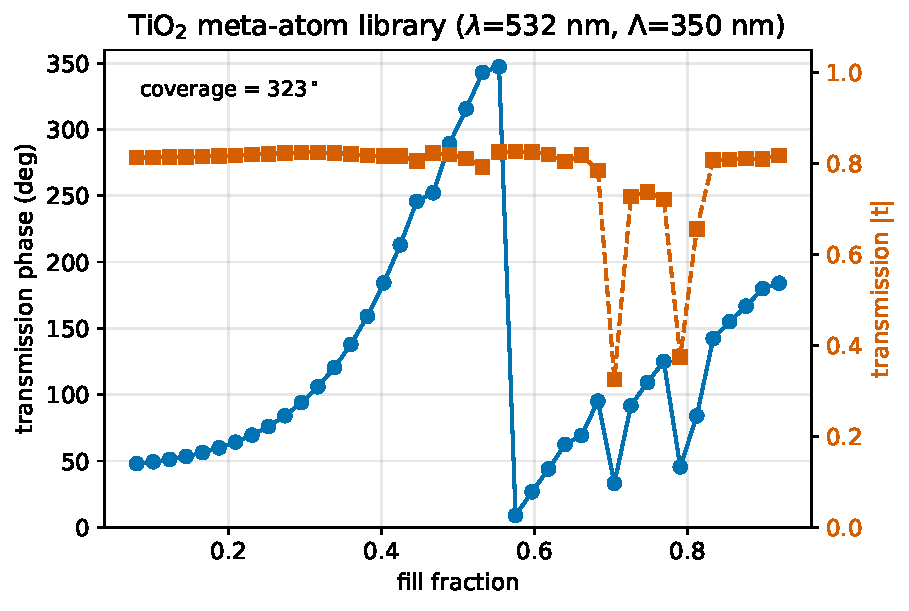
\includegraphics[width=0.8\textwidth]{figures/fig_library.pdf}
\caption{Meta-atom phase library: transmission phase and amplitude $|t|$ vs pillar fill
for a TiO$_2$ square pillar ($\lambda = 532$~nm, $\Lambda = 350$~nm, $H = 600$~nm).}
\label{fig:library}
\end{figure}

\begin{figure}[t]
\centering
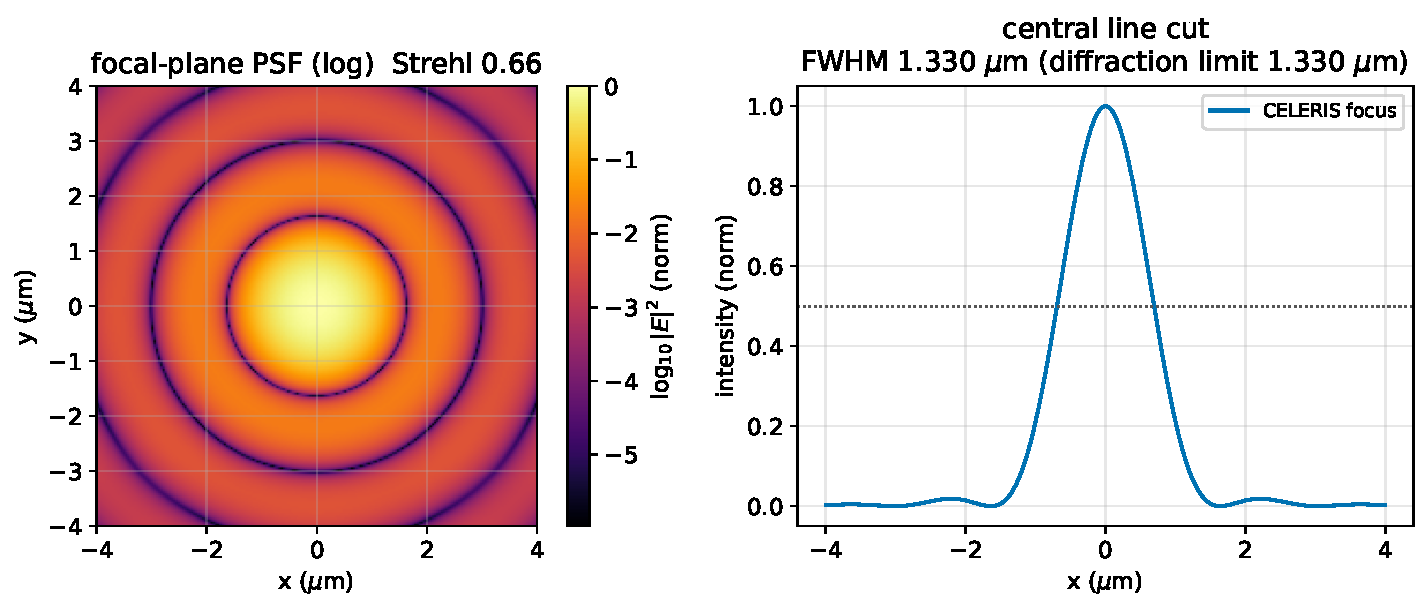
\includegraphics[width=\textwidth]{figures/fig_psf.pdf}
\caption{Focal-plane PSF of the designed lens (log scale, left) and its central line
cut (right): FWHM $= 1.330~\mu$m, exactly the diffraction limit $\lambda f/D$.}
\label{fig:psf}
\end{figure}

The full pipeline is demonstrated by reproducing two canonical published devices end
to end:
\begin{itemize}
\item Khorasaninejad et al., \emph{Science} \textbf{352}, 1190 (2016)
      \cite{khorasaninejad2016} --- an NA${=}0.80$ Pancharatnam--Berry TiO$_2$ nanofin
      metalens. CELERIS solves the published nanofin geometry with the deposited
      ALD-TiO$_2$ optical constants and recovers near-ideal half-wave-plate behavior
      (transmitted-normalized conversion 96--99\%), an exact geometric phase, and a
      diffraction-limited focal spot.
\item Chen et al., \emph{Nat.\ Nanotechnol.} \textbf{13}, 220 (2018) \cite{chen2018}
      --- a broadband achromatic visible metalens. CELERIS reproduces the central
      physical limit (the required group-delay span sits at the ${\sim}5$~fs
      single-nanofin ceiling, so the aperture is group-delay-limited) and, via
      single-etch group-delay engineering on a birefringent Pancharatnam--Berry library,
      flattens the chromatic focal shift relative to a dispersion-blind lens built from
      the same library (Fig.~\ref{fig:achromatic}).
\end{itemize}

\begin{figure}[t]
\centering
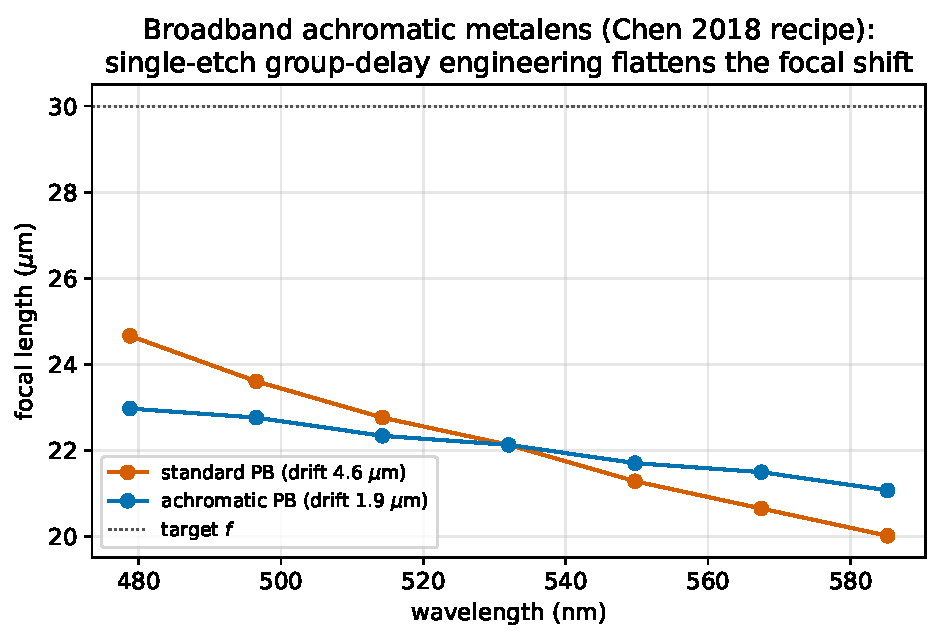
\includegraphics[width=0.8\textwidth]{figures/fig_achromatic.pdf}
\caption{Broadband achromatic metalens (Chen 2018 recipe): rigorous focal length vs
wavelength for a standard Pancharatnam--Berry lens and a group-delay-engineered
achromatic lens built from the \emph{same} single-etch birefringent library.
Group-delay matching flattens the chromatic focal shift (drift $4.6 \to 1.9~\mu$m).
At this small demonstration aperture ($D = 10~\mu$m, low Fresnel number) the
\emph{absolute} focus of both designs sits below the geometric target $f$; the effect
shown is the \emph{relative} achromatic flattening, which is what the group-delay
objective controls.}
\label{fig:achromatic}
\end{figure}

%% ---------------------------------------------------------------------------
\section{Performance}
The GPU accelerates far-field propagation only; the RCWA modal solve runs on the CPU.
We benchmark the propagation kernel (single precision) against CELERIS's own optimized
16-core CPU propagation (\texttt{compute\_psf}, double precision) using the built-in
\texttt{psfbench} command on an RTX~4070 laptop GPU. Results agree to machine precision
(max$|\Delta$ normalized PSF$| = 0$). Measured speedups (GPU vs 16-core CPU) are given
in Table~\ref{tab:perf}.

\begin{table}[t]
\centering
\caption{Far-field propagation: GPU (RTX~4070 laptop) vs optimized 16-core CPU.}
\label{tab:perf}
\begin{tabular}{lccccc}
\toprule
Aperture (pillars) & Focal grid & CPU & GPU & Speedup \\
\midrule
92\,k  & $161^2$  & 178--202~ms & 35--37~ms & \textbf{4.8--5.8$\times$} \\
92\,k  & $321^2$  & 274~ms      & 140~ms    & 2.0$\times$ \\
92\,k  & $641^2$  & 666~ms      & 519~ms    & 1.3$\times$ \\
92\,k  & $1024^2$ & 1457~ms     & 1312~ms   & 1.1$\times$ \\
256\,k & $161^2$  & 241~ms      & 111~ms    & 2.2$\times$ \\
577\,k & $161^2$  & 434~ms      & 252~ms    & 1.7$\times$ \\
\bottomrule
\end{tabular}
\end{table}

So on this hardware the GPU gives a modest ${\sim}1$--$6\times$ over a well-parallelized
16-core CPU, not the order-of-magnitude win a naive single-threaded baseline would
suggest. The speedup \emph{decreasing} with grid size indicates the current kernel is
memory-bound (each thread re-reads the full pillar list from global memory);
shared-memory tiling is a clear future optimization. We report these numbers rather than
a headline figure precisely because an apples-to-apples multicore comparison is the
honest one.

The dominant cost, however, is the RCWA modal solve, not propagation. The solve is
bounded by dense complex linear algebra (operator assembly, matrix inverses, and the
S-matrix recursion), which an optional Intel MKL backend accelerates. Because CELERIS
parallelizes its unit-cell sweeps across cores itself, MKL is pinned to a single thread
to avoid nested oversubscription; composed this way it is $2.3\times$ faster than the
AVX2 build on an $M=8$ metalens library design (5.9~s vs 13.5~s, 16-core), with larger
gains at higher Fourier order. The default build has no MKL dependency (header-only
Eigen with AVX2); MKL is opt-in.

%% ---------------------------------------------------------------------------
\section{Limitations}
\begin{itemize}
\item \textbf{The RCWA eigensolve is CPU-only.} The GPU accelerates far-field
      propagation, not the modal solve. A GPU eigensolve was prototyped (cuSOLVER) and
      found no faster than the CPU path; the promising direction is batching the many
      independent unit-cell solves of a library, which is future work.
\item \textbf{Inverse design uses finite-difference optimization} over low-dimensional
      parametric meta-atoms; an analytic adjoint (true gradient-based / differentiable
      RCWA) is planned.
\item \textbf{Curved shapes (circle/ellipse) converge slowly} (staircasing of a curved
      interface), a known RCWA property confirmed against \texttt{grcwa}.
\item \textbf{Achromatic multi-height designs imply a grayscale/multi-level etch}; the
      single-etch Pancharatnam--Berry variant is the directly fabricable one.
\item \textbf{Scope is metalenses/metasurfaces via RCWA} --- explicitly not FDTD or ray
      tracing.
\end{itemize}

%% ---------------------------------------------------------------------------
\section*{Declaration of generative AI in the writing process}
During the preparation of this work the author used Anthropic Claude to assist with
software implementation and manuscript drafting. The author reviewed and edited all
output, made every design and physics decision, and takes full responsibility for the
content; all numerical results are enforced by the validation suite described above.

%% ---------------------------------------------------------------------------
\bibliographystyle{elsarticle-num}
\bibliography{paper}

\end{document}
